\chapter{Applications}

This section provides practical examples through which this extension shows itself to be useful and relevant in fulfilling its purpose of detecting vulnerabilities in websites. Firstly, we will demonstrate how the \textit{Recommendations} feature can be used as a low effort entry point into analysing websites for potential vulnerabilities. Secondly, we will use our Test Harness to demonstrate the uses of the \textit{Action Replay} feature in tweaking and replaying innocent requests to produce behaviour that exposes vulnerabilities on a website. We then show how the \textit{Passive Mode} behaves by showcasing how it performs against the intentionally vulnerable test page. Each of these sections will begin with a preamble covering how the example we will go through is vulnerable to establish a better understanding on how the extension exposes said vulnerability. Finally, we run through a case study of a live website vulnerability that we discovered and exploited as a result of using the extension on it.

\section{Recommendations} \label{applications_recommendations}

In order to set up the example to demonstrate a use case of the \textit{Recommendations}, we set up the Test Harness with 2 intentional XSS Vulnerabilities that work in the same way - any input that is submitted in either the \texttt{injection} or \texttt{injection2} input fields is reflected on the page below its respective input (in the \texttt{output} and \texttt{output2} fields respectively). The source code of the page at this point is shown in Listing \ref{lst:test_harness}, and the resulting rendered page is shown in Figure \ref{fig:test_harness_default}. \\


%\begin{minipage}{\linewidth}
\begin{lstlisting}[label={lst:test_harness}, language={HTML}, caption={The HTML contents of the Test Harness for this example. Two of the inputs in the page are reflected onto the page when they are submitted as query parameters (i.e. seen in the page URL)}]
<script>
	window.onload = function() {
		var url = new URL(window.location.href);
		
		var c = url.searchParams.get("injection");
		if (c) {
			document.getElementById("output").innerHTML = c;
		}
		
		var d = url.searchParams.get("injection2");
		if (d) {
			document.getElementById("output2").innerHTML = d;
		}
	}
</script>

<h1>Vulnerability Testing page</h1>

<form id="boop" action="">
	<input type="text" name="injection" value=""/>
	<input type="text" name="unused" value="">
	<input type="submit">
</form>
<h2 id="output"></h2>

<form id="beep" action="">
	<input type="text" name="unused" value=""/>
	<input type="text" name="injection2" value="">
	<input type="submit">
</form>
<h2 id="output2"></h2>
\end{lstlisting}
%\end{minipage}



\begin{figure}[h]
	\centering
	\begin{subfigure}{.45\textwidth}
		\centering
		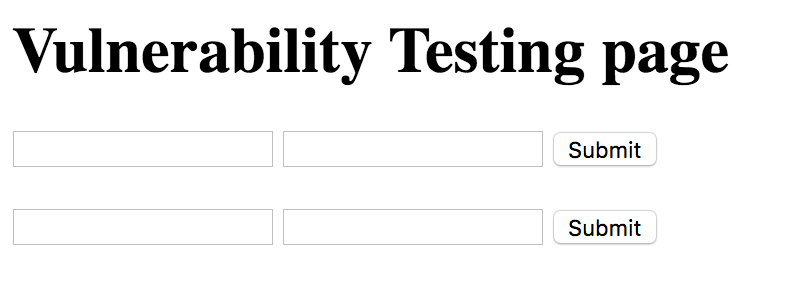
\includegraphics[width=.8\linewidth]{images/test_harness_recommendations.png}
		\label{fig:test_harness_original}
	\end{subfigure}%
	\begin{subfigure}{.6\textwidth}
		\centering
		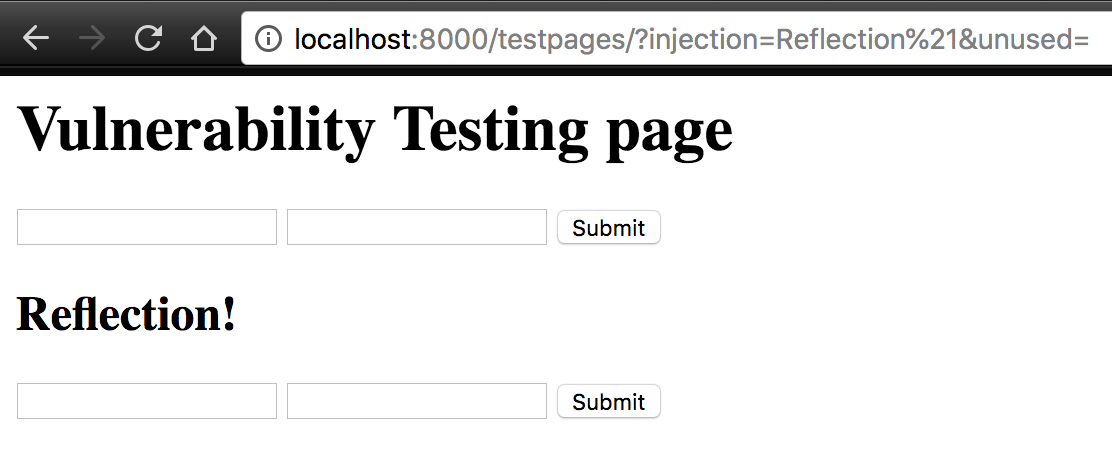
\includegraphics[width=.8\linewidth]{images/test_harness_reflection_1.png}
		\label{fig:test_harness_reflection_1}
	\end{subfigure}
	\caption{The default Test harness page to demonstrate XSS vulnerabilities. Submitting the first input causes the reflection in the second image.}
	\label{fig:test_harness_default}
\end{figure} 

Now we enable the recommendations in this page - setting the sensitivity parameter to \textbf{1}. At this stage, one input is added per form on the page, encouraging the user to "investigate" the first input on each of the forms, seen in \ref{fig:test_harness_recommendations_2}. 

\begin{figure}[h]
	\centering
	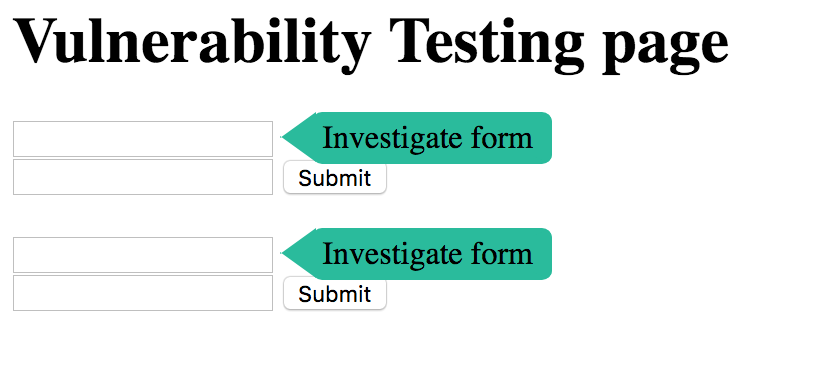
\includegraphics[width=0.7\textwidth]{images/test_harness_recommendations_2.png}
	\caption{Enabling the recommendations on the Test Harness}
	\label{fig:test_harness_recommendations_2}
\end{figure}

If the user decides to test the first input on the page, one of the attempted attacks will inject the following into the input:

\begin{center}
	\texttt{<img src=a onerror="window.location.replace( 'chrome-extension://ID/request\_logger.html?ref=CURRENT\_URL')">}
\end{center}

where the \texttt{ID} parameter is replaced by the ID given by Chrome to the extension, and the \texttt{CURRENT\_URL} is the current web address before the form was submitted. This is an example of an XSS attack which surreptitiously executes Javascript on a page by injecting an \texttt{<img>} tag with an invalid source location. This triggers an error when the image is later loaded on that page (since we have established that this input is reflected back onto the page). At this point, the \texttt{onerror} callback given to the input is executed, and in our case, will change the location of the current page to our previously mentioned \texttt{request\_logger} page, passing the current URL as a query parameter in this referral. \\


The \texttt{request\_logger} page is equipped to deal with this specific type of request, by alerting the user both through the extension and in the page output that an XSS vulnerability has been found, indicating the address of the culprit page. The only (current) means to reach this page in the extension is through the payloads prepared in the attacks, meaning that Javascript had to have been executed by one of these, thus indicating an XSS vulnerability. Upon opening the extension for further details, the initial Test Harness URL is then listed as a website vulnerable to XSS. \\


\begin{figure}[h]
	\centering
	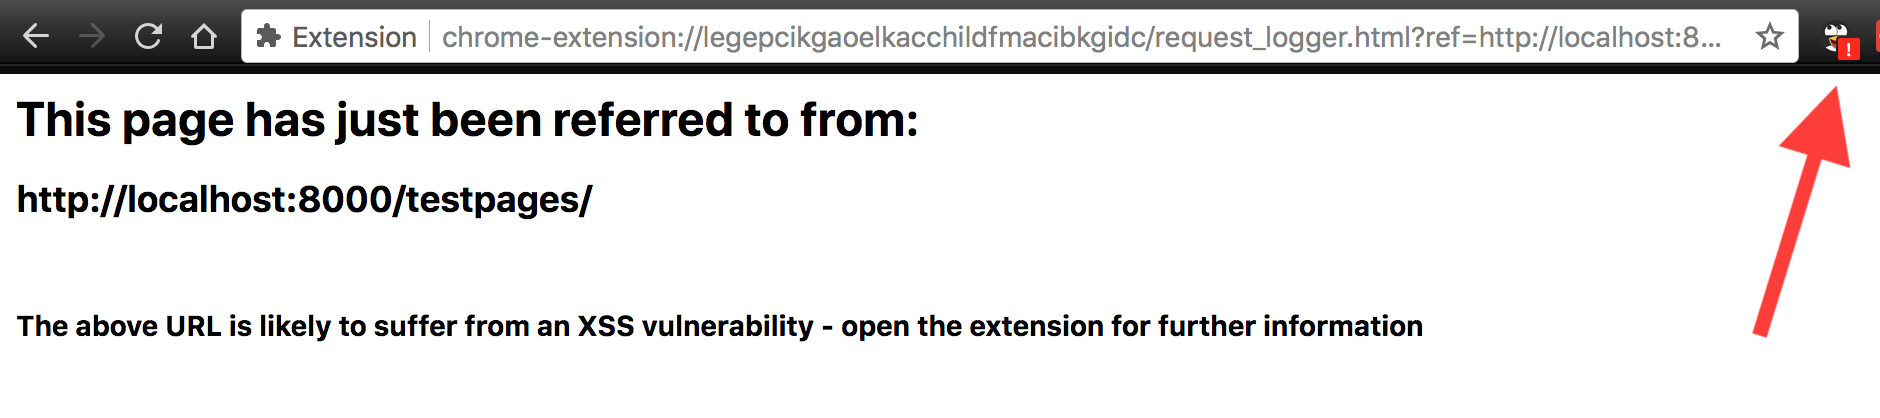
\includegraphics[width=	\textwidth]{images/request_logger_warning.png}
	\caption{The request logger page warns the user that the reason they've reached this page is likely to have been due to an XSS vulnerability. Note that the extension badge is also updated with a warning \textbf{(!)} label to indicate this (arrow added in diagram for emphasis).}
	\label{fig:request_logger_warning}
\end{figure}

\begin{figure}[h]
	\centering
	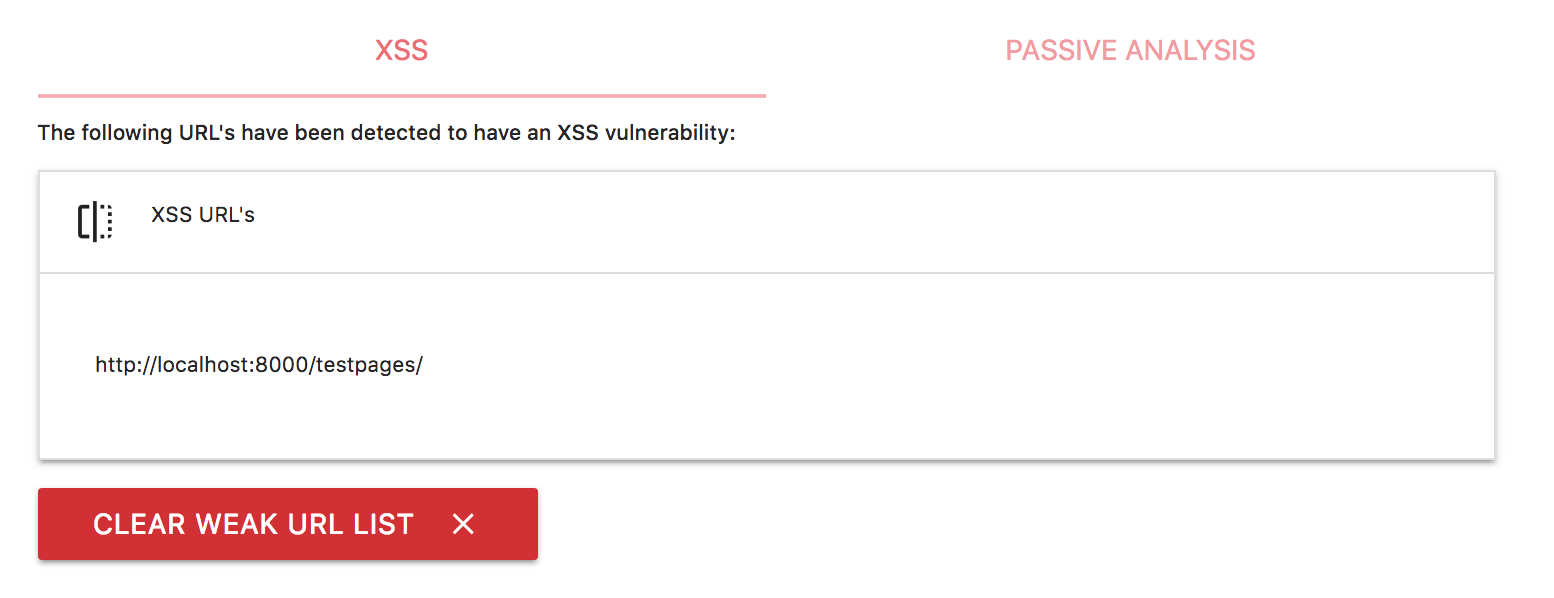
\includegraphics[width=	\textwidth]{images/xss_vulnerable_url.png}
	\caption{Opening the extension confirms that the suspicious URL was indeed vulnerable to XSS.}
	\label{fig:xss_vulnerable_url}
\end{figure}


\section{Action Replay}

Now we consider how we can use the Action Replay algorithm to automatically replay attacks on focussed inputs and requests. \\

The vulnerability in this example is the same as the one from the \textit{Recommendations} section (\ref{applications_recommendations}) - the website suffers from a reflected XSS vulnerability. In this case however, we assume that through use of the website the user has noticed this, and attempts to exploit the website. Perhaps they attempt a similar injection as before to test their hypothesis:

\begin{center}
	\texttt{<img src=a >} 
\end{center}

Upon trying this input, this is the page they are confronted with:

\begin{figure}[h]
	\centering
	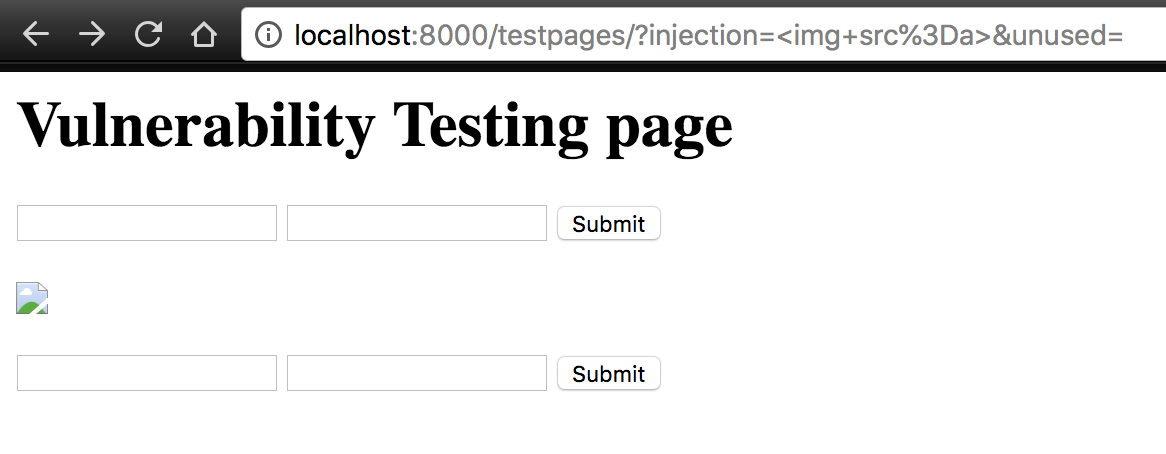
\includegraphics[width=0.7\textwidth]{images/action_replay_initial.png}
	\caption{Injecting \texttt{<img src=a>} into an input results in this page}
	\label{fig:action_replay_initial}
\end{figure}

To a web security analyst with a more trained eye, this may present a security risk, as they were freely able to inject a HTML tag into the page of their choosing. It is at this point where they decide to focus on this particular input and activate the Action Replay. After enabling and starting a recording, they reattempt the earlier injection. \\

\begin{figure}[h]
	\centering
	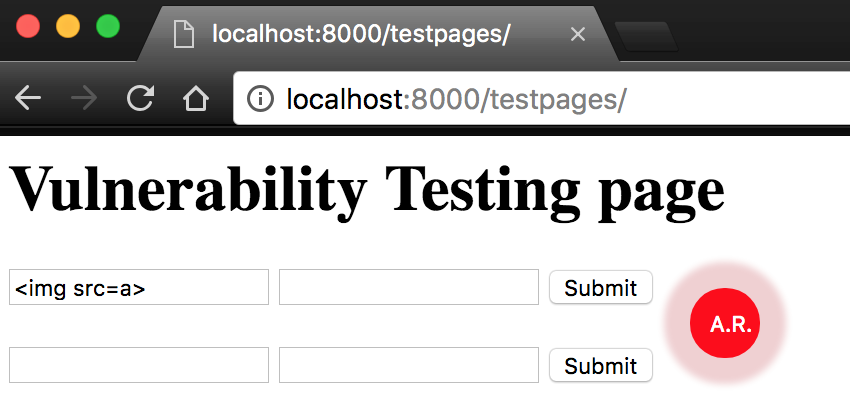
\includegraphics[width=0.7\textwidth]{images/action_replay_attack.png}
	\caption{Retrying the attack while recording using Action Replay}
	\label{fig:action_replay_attack}
\end{figure}

Once the new page loads, the user can then stop the recording by clicking the \textit{AR} button once again. At this point, the analysis and automated replay begins. If the algorithm has appropriately detected a set of potentially dangerous inputs it can override to begin an attack, then almost immediately after finishing the recording, Chrome will open several new windows, each of which attempts an attack. Not all of these are expected to yield successful vulnerability identifications, but, for this example, we see that one of the resultant tabs has ended up in the \textit{Request Logger} page. This can only indicate that the payload of one of the attacks was successful. \\ 


\begin{figure}[h]
	\centering
	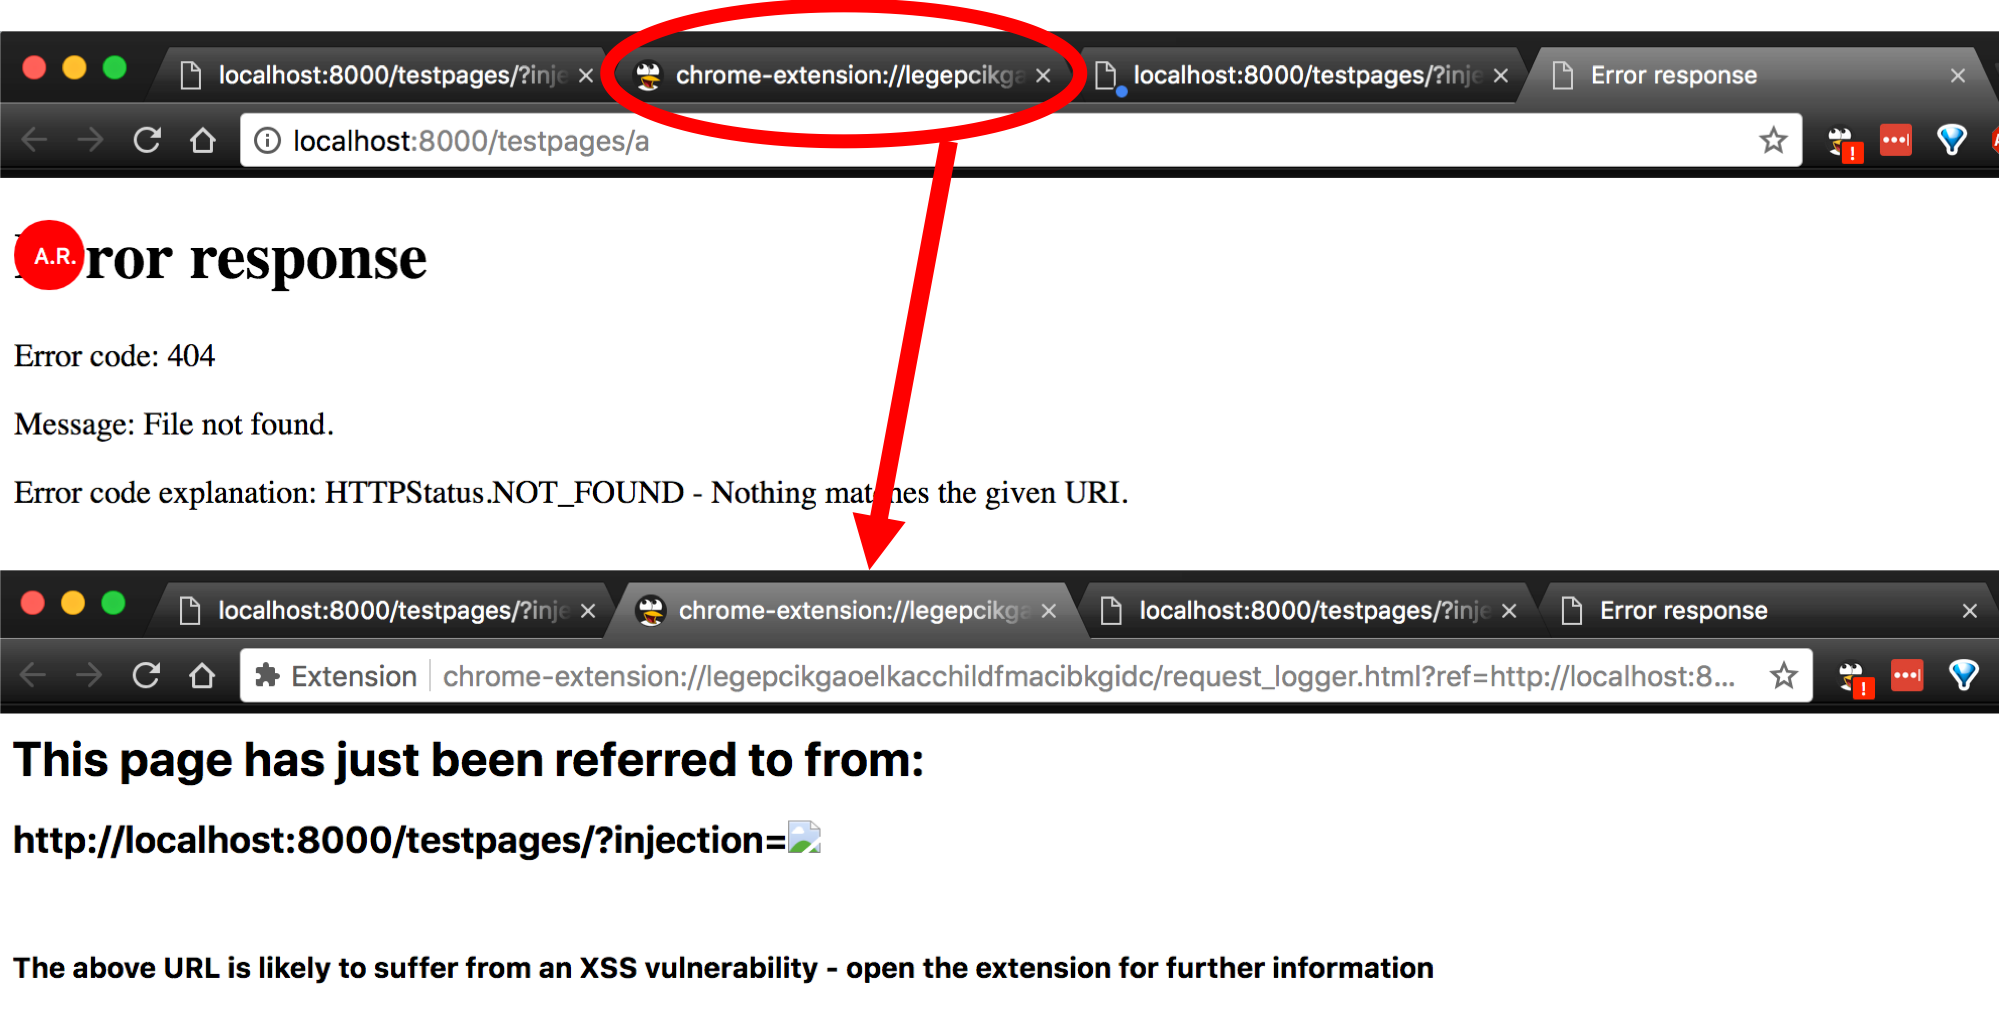
\includegraphics[width=\textwidth]{images/successful_replay.png}
	\caption{The Action Replay generates the outputs of several attacks in new windows. The 2nd of the inspected windows showcases a successfully detected vulnerability that executed a Javascript payload.}
	\label{fig:successful_replay}
\end{figure}

As before, once this stage is reached, we have the appropriately reported information in the extension. The list of URLs that suffer from XSS vulnerabities is updated, containing the latest victim. Additionally, Action Replay publishes a list of inputs it considered to be dangerous, showing the user which inputs were targeted by the automated attacks.  \\

\begin{figure}[h]
	\centering
	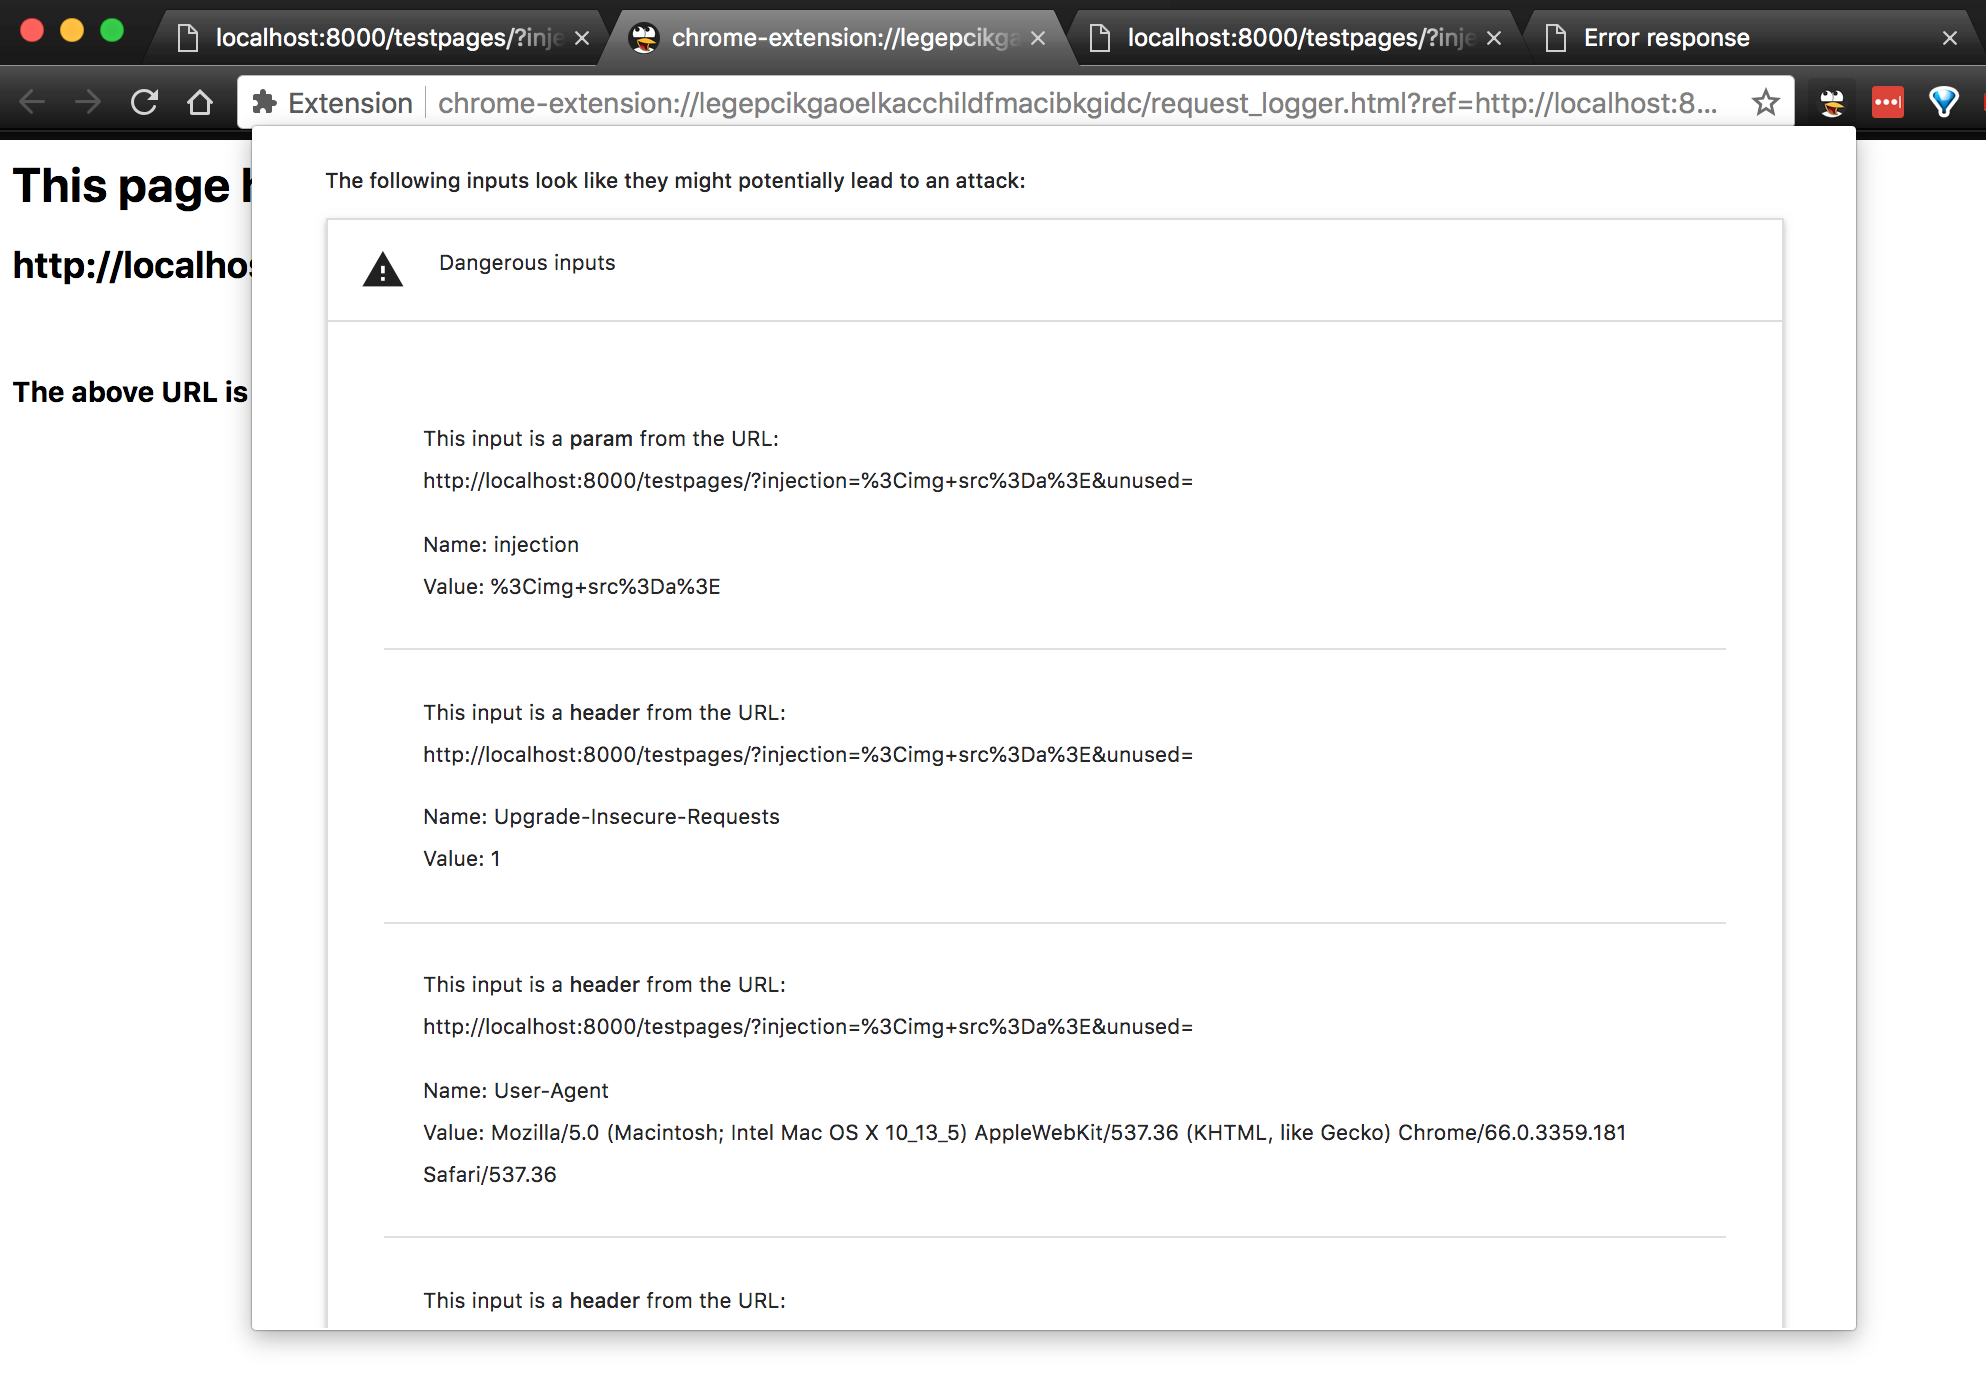
\includegraphics[width=\textwidth]{images/dangerous_inputs.png}
	\caption{The Action Replay outputs a list of inputs it has considered to be dangerous. In this screenshot, we see the \textbf{param} with the name \textbf{injection} is one of the potentially dangerous inputs. }
	\label{fig:dangerous_inputs}
\end{figure}





\section{Passive Mode}


\section{Live Vulnerability Test Case}

http://studios.fitpass.co.in/login





















